
%%%%%%%%%%%%%%%%%%%%%%%%%%%%%%%%%%%%%%%%%%%%%%%%%%%%%%%%%
%Eddy current model
\section{The eddy-current model and asymptotic expansion}\label{sect:eddycurrent}

We briefly discuss the eddy-current model along with stating the asymptotic expansion that forms the basis of the magnetic polarizability description of conducting objects in metal detection.
\subsection{Eddy-current model}
The eddy current model is a low frequency approximation of the Maxwell system that neglects the displacement currents, which is valid when the frequency is small and the conductivity of the body is high. A rigorous justification of the model involves the topology of the conducting body~\cite{ammaribuffa2000}.  The eddy current model is described by the system

\begin{subequations}\label{Eddy Current}
\begin{align}
\nabla\times\bm{E}_{\alpha}&=\im \omega\mu\bm{H}_{\alpha},\\
\nabla\times\bm{H}_{\alpha}&=\bm{J}_0+\sigma\bm{E}_{\alpha}.
\end{align}
\end{subequations}
where $\bm{E}_{\alpha}$ and $\bm{H}_{\alpha}$ are the electric and magnetic interaction fields, respectively, $ \bm{J}_0$ is an external current source, $\im:=\sqrt{-1}$, $\omega$ is the angular frequency, $\mu$ is the magnetic permeability and $\sigma$ is the electric conductivity.  We will use the eddy current model for describing the forward and inverse problems in the metal detection problem.

\subsubsection{Metal Detection Forward Problem} \label{sect:forward}
In the forward (or direct) problem, the position and materials of the conducting body $B_{\alpha}$ are known. The object has a high conductivity, $\sigma=\sigma_*$, and a permeability, $\mu=\mu_*$. The conducting body is assumed to buried in soil, which is assumed to be of a much lower conductivity so that $\sigma\approx0$ and have a permeability $\mu=\mu_0:= 4 \pi \times 10^{-7}\text{H/m}$. A background field is generated by a solenodial current source $\bm{J}_0$ with support in the air above the soil, which has $\sigma=0$ and $\mu =\mu_0$. The region around the object is $B_{\alpha}^c\vcentcolon=\mathbb{R}^3\setminus B_{\alpha}$as shown  in Figure \ref{metal detection}.

%Model setup diagram
\begin{figure}[H]
\begin{center}
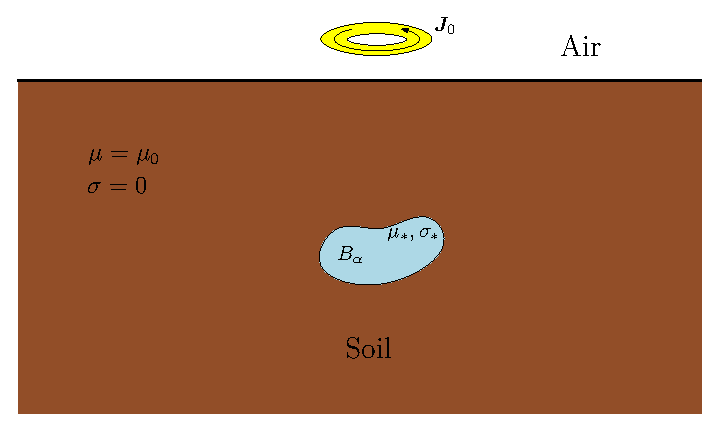
\includegraphics[width=0.7\textwidth, keepaspectratio]{Figures/MetalDetectionSoilSmall.eps}
\caption{A diagram showing a hidden conducting object $B_{\alpha}$ surrounded by it's compliment $B_{\alpha}^c$ which is made up of soil and air.}
\label{metal detection}
\end{center}
\end{figure}
The forward model is described by the system (\ref{Eddy Current}),  which hold in ${\mathbb R}^3$, with
\begin{align}
\mu (\bm{x}) = \left \{  \begin{array}{ll} \mu_* & \bm{x} \in B_{\alpha} \\
\mu_0 & \bm{x} \in B_{\alpha}^c \end{array} \right . ,
\sigma (\bm{x}) = \left \{  \begin{array}{ll} \sigma_* & \bm{x} \in B_{\alpha} \\
0 & \bm{x} \in B_{\alpha}^c \end{array} \right .,
\end{align}
and the regions $B_\alpha$  and $B_\alpha^c $ are coupled by the transmission conditions
\begin{align}
\left [\bm{n} \times \bm{E}_\alpha\right ]_{\Gamma_{\alpha}}=\left [\bm{n} \times \bm{H}_\alpha\right ]_{\Gamma_{\alpha}}=\bm{0},\label{jump}
\end{align}
\noindent
which hold on  $\Gamma_\alpha:= \partial B_\alpha$. In the above, $[u ]_{\Gamma_{\alpha}}:= u| _+ - u|_-  $ denotes the jump,  the $+$ refers to just outside of $B_\alpha$ and the $-$ to just inside and $\bm{n}$ denotes a unit outward normal to  $\Gamma_{\alpha}$. 

The electric interaction field in  (\ref{Eddy Current}) is non-physical and, to ensure uniqueness of this field, the condition $\nabla \cdot \bm{E}_\alpha =0$ is imposed in $B_\alpha^c$. Furthermore,  we also require that $\bm{E}_{\alpha}=O(1/|\bm{x}|)$ and $\bm{H}_{\alpha}=O(1/|\bm{x}|)$  as $|\bm{x} | \to \infty$, denoting that the fields go to zero at least as fast as $1/|\bm{x}|$, although, in practice, this can faster.


\subsubsection{Metal Detection Inverse Problem} \label{sect:inverseproblem}
In the metal detection inverse problem, one wishes to determine the location, shape and material properties of the conducting object $B_\alpha$, described above, from measurements of $(\bm{H}_\alpha - \bm{H}_0) (\bm{x})$ at locations $\bm{x}$ in the air. Here, $\bm{H}_0$ denotes the background magnetic and is the magnetic field that result from the solution of (\ref{Eddy Current}) without the presence of the object $B_\alpha$, i.e.  $\bm{E}_0$ and $\bm{H}_0$ are the solution of (\ref{Eddy Current}) with $\sigma =0$ and $\mu=\mu_0$ in ${\mathbb R}^3$. Similar to above, we also require that $\bm{E}_{0}=O(1/|\bm{x}|)$ and $\bm{H}_{0}=O(1/|\bm{x}|)$  as $|\bm{x} | \to \infty$, denoting that the fields go to zero at least as fast as $1/|\bm{x}|$, although, in practice, this can faster.

Practical metal detectors measure a voltage perturbation, which corresponds to $\int_S \bm{n} \cdot (\bm{H}_\alpha - \bm{H}_0) (\bm{x}) \dif \bm{x}$ over an appropriate surface $S$~\cite{LedgerLionheart2018}. For very small coils, this voltage perturbation corresponds to $\bm{m} \cdot (\bm{H}_\alpha - \bm{H}_0) (\bm{x})$ where $\bm{m}$ is magnetic dipole moment of the coil~\cite{LedgerLionheart2018}.



\subsection{The asymptotic expansion}
The forward problem described in Section~\ref{sect:forward}, implies that if we know $B_\alpha$ ,$ \sigma_*$ and $\mu_*$ we can solve (\ref{Eddy Current})  to determine $\bm{E}_\alpha$ and $\bm{H}_\alpha$. However, to do this repeatably for each new object is computationally expensive. Instead, we seek an approximation in the form of trying approximate the perturbation $(\bm{H}_{\alpha}-\bm{H}_0)( \bm{x})$ at some point $\bm{x}$ exterior to $B_\alpha$.

To do this, following~\cite{Ammari2014,LedgerLionheart2015} we define $B_\alpha := \alpha B + \bm{z}$ where $B$ is a unit size object, $\alpha$ is the object size and $\bm{z}$ is the object's translation from the object as shown in Figure ~\ref{BAlphaShifted}.
\begin{figure}[H]
\begin{center}
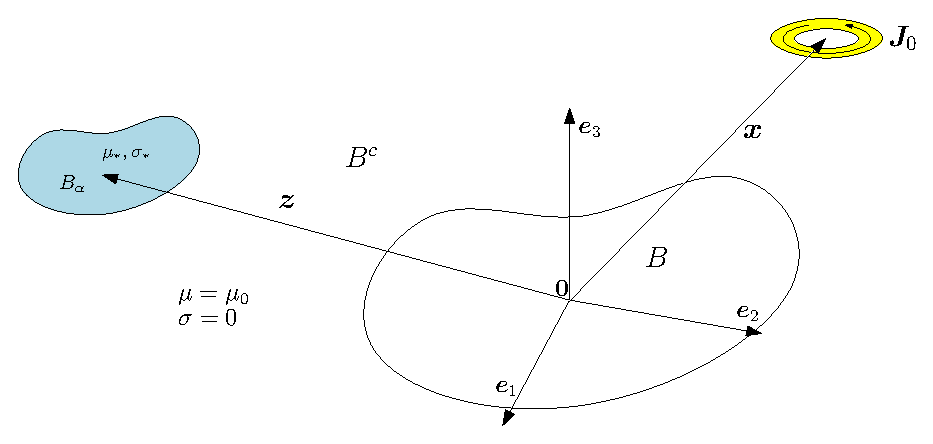
\includegraphics[width=0.8\textwidth, keepaspectratio]{Figures/BAlphaShifted.eps}
\caption{A diagram showing the physical description of $B_{\alpha}$ with respect to the coordinate axes.}
\label{BAlphaShifted}
\end{center}
\end{figure}
\noindent Then, using results obtained by Ammari, Chen, Chen, Garnier and Volkov~\cite{Ammari2014}, Ledger and Lionheart~ \cite{LedgerLionheart2015} have derived the
 asymptotic expansion 
%Asymptotic formula
\begin{align}
(\bm{H}_{\alpha}-\bm{H}_0)(\bm{x})_i=(\bm{D}_{\bm{x}}^2G(\bm{x},\bm{z}))_{ij}(\mathcal{M})_{jk}(\bm{H}_0(\bm{z}))_k+O(\alpha^4), \label{eqn:asymp}
\end{align}
which holds as $\alpha\to 0$. In the above, $G(\bm{x} ,\bm{z}  ) = 1/ {4\pi | \bm{x} -\bm{z} |}$ is the free space Laplace Green's function, $ \bm{D}^2_x G$ denotes the Hessian of $G$ and Einstein summation convention of the indices is implied. The term ${\mathcal M}$ is the symmetric rank 2 magnetic polarizability tensor, which describes the shape and material properties of the object $B_\alpha $ and is independent of the object's position, but is frequency dependent. We will sometimes write $\mathcal{M}[ \alpha B, \omega ]$ to emphasise this. The above formulation, and the definition of ${\mathcal M}$ below, are presented for the case of a single homogenous object $B$, the extension to multiple inhomogeneous objects can be found in~\cite{LedgerLionheartamad2019,LedgerLionheart2019}.

%presented in \cite{LedgerLionheart2015} since it evaluates the object by means of a complex symmetric rank 2 tensor which is invariant relative to position in the field. The expansion also includes an error term, giving a measure of the accuracy of the approximation and is given as follows. We may evaluate the perturbation $(\bm{H}_{\alpha}-\bm{H}_0)$ at the point $\bm{x}$ caused by the object $B_{\alpha}$ as,
%
%which holds as $\alpha\rightarrow 0$. Let us also note the term $\bm{R}(\bm{x})=O(\alpha^4)$ which is the error term we mentioned before. It is also useful for us to note at this point our physical description of $B_{\alpha}$, we define $B_{\alpha}=\alpha B+\bm{z}$ a unit sized object $B$ scaled by $\alpha$ and translated by $\bm{z}$ shown in Figure \ref{BAlphaShifted}.
%B\alpha diagram

\noindent
Let us now turn our attention to the computation of the coefficients of $\mathcal{M}$ in (\ref{eqn:asymp}), which describes the shape and material properties of $B_\alpha$. From the following, will be able compute a library of such tensors for different choices of $\alpha B$ since ${\mathcal M}$ is independent of ${\bm z}$, this, in turn, will lend itself to the application of dictionary based classification algorithms~\cite{LedgerLionheartamad2019} for the solution of the inverse problem stated in Section~\ref{sect:inverseproblem}.


\subsection{Calculating the Magnetic Polarizability Tensor}\label{sectCalculatingMPT}
In the following, we state the explicit formulae for the computation of the coefficients of $\mathcal{M}$, which have been derived in~\cite{LedgerLionheart2019}.  Earlier, Ledger and Lionheart~\cite{LedgerLionheart2015,LedgerLionheart2016,LedgerLionheart2018} have also derived other equivalent formulations, but those below lead to a more natural FEM implementation (using {\texttt{NGSolve}} ).

Following~\cite{LedgerLionheart2019}, we write $\mathcal{M} = ( \mathcal{M})_{ij} \bm{e}_i  \otimes \bm{e}_j$ where $\bm{e}_i$ denotes the $i$th orthonormal unit vector and use the splitting $(\mathcal{M})_{ij}:=(\mathcal{N}^0)_{ij}+(\mathcal{R})_{ij}+\im(  \mathcal{I})_{ij}$ with
%Tensor definitions
\begin{subequations}
\label{eqn:NRI}
\begin{align}
(\mathcal{N}^0[ \alpha B] )_{ij}&:=\alpha^3\delta_{ij}\int_{B}(1-\mu_r^{-1})\dif \bm{\xi}+\frac{\alpha^3}{4}\int_{B\cup B^c}\tilde{\mu}_r^{-1}\nabla\times\tilde{\bm{\theta}}_i^{(0)}\cdot\nabla\times\tilde{\bm{\theta}}_j^{(0)}\ \dif \bm{\xi},\\
(\mathcal{R}[\alpha B, \omega])_{ij}&:=-\frac{\alpha^3}{4}\int_{B\cup B^c}\tilde{\mu}_r^{-1}\nabla\times\bm{\theta}_j^{(1)}\cdot\nabla\times\overline{\bm{\theta}_i^{(1)}}\ \dif \bm{\xi},\\
(\mathcal{I}[\alpha B, \omega])_{ij}&:=\frac{\alpha^3}{4}\int_B\nu\Big(\bm{\theta}_j^{(1)}+(\tilde{\bm{\theta}}_j^{(0)}+\bm{e}_j\times\bm{\xi})\Big)\cdot\Big(\overline{\bm{\theta}_i^{(1)}+(\tilde{\bm{\theta}}_i^{(0)}+\bm{e}_i\times\bm{\xi})}\Big)\ \dif \bm{\xi}.
\end{align}
\end{subequations}
In the above,
\begin{align}
\tilde{\mu}_r ( \bm{\xi} ) := \left \{ \begin{array}{ll}  \mu_r :=\mu_*/\mu_0 & \bm{\xi} \in B\\
1 & \bm{\xi} \in B^c \end{array} \right . \nonumber,
\end{align}
and $\nu:=\alpha^2\omega\mu_0\sigma_*$, $\delta_{ij}$ is the Kronecker delta and the overbar denotes the complex conjugate. The computation of (\ref{eqn:NRI}) rely on the solution of the transmission problems~\cite{LedgerLionheart2019}
\begin{subequations}
\label{eqn:Theta0}
\begin{align}
\nabla\times\tilde{\mu}_r^{-1}\nabla\times\bm{\theta}_i^{(0)}&=\bm{0} &&\textrm{in }B\cup B^c,\\
\nabla\cdot\bm{\theta}_i^{(0)}&=0 &&\textrm{in }B\cup B^c,\\
[{\bm{n}}\times\bm{\theta}_i^{(0)}]_{\Gamma}&=\bm{0} &&\textrm{on }\Gamma,\\
[{\bm{n}}\times\tilde{\mu}_r^{-1}\nabla\times\bm{\theta}_i^{(0)}]_{\Gamma}&=\bm{0} &&\textrm{on }\Gamma,\\
\bm{\theta}_i^{(0)}-{\bm{e}}_i\times\bm{\xi}&=\bm{O}(|\bm{\xi}|^{-1}) &&\textrm{as }|\bm{\xi}|\rightarrow\infty,
\end{align}
\end{subequations}
and 
%Theta 1 transmission problem
\begin{subequations}
\label{eqn:Theta1}
\begin{align}
\nabla\times\mu_r^{-1}\nabla\times\bm{\theta}_i^{(1)}-\im \nu  (\bm{\theta}_i^{(0)}+\bm{\theta}_i^{(1)})&=\bm{0}&&\textrm{in }B,\\
\nabla \times \nabla \times \bm{\theta}_i^{(1)} &= \bm{0} && \text{in }B^c,\\
\nabla\cdot\bm{\theta}_i^{(1)}&=0&&\textrm{in }B^c,\\
[{\bm{n}}\times\bm{\theta}_i^{(1)}]_{\Gamma}&=\bm{0}&&\textrm{on }\Gamma,\\
[{\bm{n}}\times\tilde{\mu}_r^{-1}\nabla\times\bm{\theta}_i^{(1)}]_{\Gamma}&=\bm{0}&&\textrm{on }\Gamma,\\
\bm{\theta}_i^{(1)}(\bm{\xi})&=\bm{O}(|\bm{\xi}|^{-1})&&\textrm{as }|\bm{\xi}|\rightarrow\infty.
\end{align}
\end{subequations}
Note also that $\tilde{\bm{\theta}}_i^{(0)}\vcentcolon=\bm{\theta}_i^{(0)}-\hat{\bm{e}}_i\times\bm{\xi}.$ In order to obtain a discrete approximation using the FEM, we need to introduce a finite computational domain $\Omega$ such that $B\subset\Omega$, whose boundary $\partial\Omega$ is placed sufficiently far from the object $B$. 

The tensor $\mathcal{N}^0[ \alpha B] $ describes the magnetostatic characterisation of $\alpha B$ and is independent of $\omega$. The frequency dependent $\mathcal{R}[\alpha B, \omega]$ tensor vanishes at low frequency and $\mathcal{N}^0[\alpha B]+\mathcal{R}[\alpha B , \omega] =\text{Re}( {\mathcal M} [ \alpha B, \omega]) $ describes the frequency behaviour of the real part of the tensor. Similarly, $\mathcal{I}[\alpha B, \omega] = \text{Im}( {\mathcal M} [ \alpha B, \omega])$ describes the frequency behaviour of the imaginary part of the tensor, which vanishes at low frequencies and  tends to $0$ as the upper limiting frequency of the eddy current model is reached~\cite{LedgerLionheart2019}.

In order to compute the tensor coefficients in (\ref{eqn:NRI}) we need to solve (\ref{eqn:Theta0}) and (\ref{eqn:Theta1}) (repeatably for each $\omega$) and this will be achieved by computing approximate solutions using a range of different numerical schemes
\begin{enumerate}

\item A $hp$ FEM discretisation of the transmission problems (\ref{eqn:Theta0}) and (\ref{eqn:Theta1}) using \texttt{NGSolve}~\cite{NGSolve,zaglmayrphd,netgendet} to compute ${\mathcal M}[\alpha B , \omega]$ for a single frequency.

\item A $hp$ FEM discretisation of the transmission problems (\ref{eqn:Theta0}) and (\ref{eqn:Theta1})  using \texttt{NGSolve}~\cite{NGSolve,zaglmayrphd,netgendet} for performing the  computation of ${\mathcal M}[\alpha B , \omega]$ over a range of frequencies.

\item A  Proper Orthogonal Decomposition (POD) reduced order model, which greatly accelerates the computation of the full order model in 2. for computing ${\mathcal M}[\alpha B , \omega]$ over a range of frequencies.

\item Certificates computed at run time, which indicate the accuracy of the POD outputs with respect to the full order solution over a range of frequencies.



\end{enumerate}

A detailed description of the numerical implementation of these schemes can be found in~\cite{wilsonledger2019}.

In particular, we advocate a $hp$ FEM discretisation using $\bm{H}(\text{curl})$ conforming elements 
for the transmission problems (\ref{eqn:Theta0}) and (\ref{eqn:Theta1}) due to the superior performance it overs over a traditional $h$-version of the FEM, in which only the mesh is refined. In the $hp$-version, the polynomial order of the elements can be increased, as well as refining the finite element grid, in order to obtain accurate solutions. In practice, it is often sufficient to generate a suitable mesh, which has local refinement around sharp edges and corners and increase the polynomial degree in order to obtain accurate solutions for the magnetic polarizability tensor coefficients. As an illustration, we present in Figure~\ref{fig:hprefinement} convergence curves of $\| {\mathcal N}_{hp}^0 - {\mathcal N}^0 \|_F / \| {\mathcal N}^0 \|_F $ and  $\| {\mathcal M}_{hp} - {\mathcal M}\|_F / \| {\mathcal M} \|_F $ computed for a conducting sphere of radius $\alpha=0.01\text{m} $, $\sigma_* =6\times10^6  \text{S/m}$, $\mu_* =1.5 \mu_0$, which has an analytical solution~\cite{Wait1951}, where $hp$ denotes the tensor coefficients obtained by a $hp$ FEM discretisation. The solutions obtained on a sequence of meshes with 12074, 22392, 26751, 48418, 54092, 123788 unstructured tetrahedral elements of order $p=0$ ($h$-refinement) are compared with those obtained on a fixed mesh of 12074 unstructured tetrahedral elements using of order $p=0,1,2,3$, in turn ($p$-refinement). We observe the downward sloping behaviour of the $p$-refinement convergence curve, which illustrates that exponential convergence is being obtained, compared to the slower algebraic rate with $h$-refinement.

\begin{figure}[H]
\begin{center}
$\begin{array}{c}
\includegraphics[width=0.5\textwidth]{GraphsAndData/hp-refinement/N0hp-refinement/N0hp-refinement.pdf} \\
\includegraphics[width=0.5\textwidth]{GraphsAndData/hp-refinement/MPThp-refinement/MPThp-refinement.pdf}
\end{array}$
\caption{Conducting sphere of radius $\alpha=0.01\text{m} $, $\sigma_* = 6\times10^6 \text{S/m}$, $\mu_* =1.5 \mu_0$: Convergence curves of $\| {\mathcal N}_{hp}^0 - {\mathcal N}^0 \|_F / \| {\mathcal N}^0 \|_F $ and  $\| {\mathcal M}_{hp} - {\mathcal M} \|_F / \| {\mathcal M} \|_F $ for $h$ and $p$ refinement}\label{fig:hprefinement}
\end{center}
\end{figure}


 The following describes the installation and use \texttt{MPT-Calculator}, which implements the above schemes.


